\chapter{Speed Advisory}\label{ch:app}

\begin{Summary}[Bibliographical Notes]
This chapter is partially based on the following paper in which the author was the principal investigator:

\cite{matthes2022selecting} \fullcite{matthes2022selecting}
\end{Summary}

\section{Introduction}

\section{Related Work}\label{sec:rw-uis}

\subsection{User Interfaces}

- State in simulations

- Visual User Interfaces
- Usability analysis by Krause et al.
- User Reviews on Traffic Pilot
- Not many "production-ready" solutions!

- Non-Visual User Interfaces
- Vibrotactile: Cespedes et al. \url{https://ieeexplore.ieee.org/abstract/document/8535027}

- User Interfaces for cyclists
- FastTrack: Personalization

- Avoiding the usage of bike-GLOSA in a non-cycling context (Transport mode detection)
- Resource/Energy impacts

\subsection{Impacts}

- Impacts on Cars
- Impacts on Cyclists
- Simulations, Real-World Impacts

\section{Concept}

During the ride, the user travels along the preselected route and obtains predictions for the upcoming signals via MQTT. Now, the speed advisory can be calculated from these predictions by estimating when a user will arrive at a signal. In turn, if a given speed is predicted to pass the traffic light at green depends on the distance to the signal. Thus, an algorithm must be established that estimates the distance to the traffic light as precisely as possible.

Once the signal's distance and the prediction have been obtained, the task is to provide the best possible speed advisory user interface. An important takeaway from the previous section is that the user interface must dynamically adapt itself to the prediction's quality and uncertainties. At the same time, it is crucial to design the speed advisory as intuitive and flexible as possible, to avoid distracting users from the real-world situation and provoking accidents.

Finally, another question is how to combine the speed advisory with the proposed in-app routing system. The proposed solution in this work is to overlay a three-dimensional map view with the speed advisory. This solution is utilized to establish a clear link between the user's route and the traffic light for which a speed advisory is displayed. However, this comes with the challenges of always displaying a suitable region of the map, automatically calculating new routes on route deviations, and correcting GNSS errors. All of these challenges must be overcome to provide an overall good user experience.

\subsection{Preliminary and Final Speed Advisory User Interfaces}

With the estimated distance to the traffic light and the obtained traffic light prediction, the speed advisory can be calculated and displayed on the user interface. Related work has identified multiple distinct user interfaces for speed recommendation: displaying a target speed, mapping the predicted states onto a speedometer, and utilizing a multi-lane projection. However, so far, there are no conclusive results that would indicate that one of these user interfaces is the most suitable. To determine the most suitable approach, all three methods are investigated.

\begin{figure}[htbp]
\centering
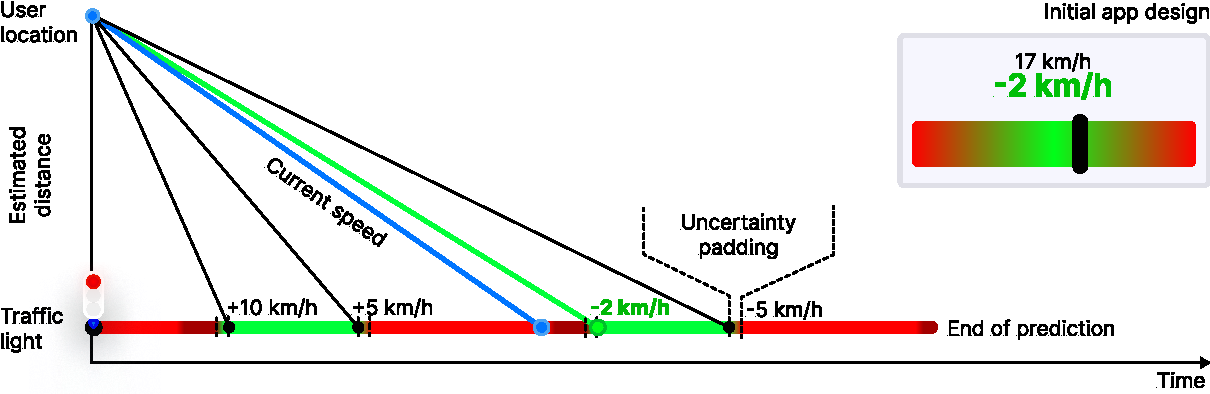
\includegraphics[width=\linewidth]{images/graph-based-speed-recommendation.pdf}
\caption{Simple speed recommendation algorithm used in initial tests.}
\label{fig:graph-based-speed-recommendation}
\end{figure}

\paragraph{Target speed recommendation:} As highlighted in \Cref{fig:graph-based-speed-recommendation}, a text-based speed recommendation is provided to the user, accompanied by a static color-coded scale indicating alignment with the green phase. This approach utilizes a simple speed recommendation algorithm developed for this purpose. The algorithm estimates the distance to the traffic light and projects the user's current speed onto predicted traffic light states, providing information about the second at which the user would reach the traffic light if they maintained their current speed. Subsequently, the algorithm checks whether the user would encounter a green phase or a red phase. If passing at a green phase is predicted, no speed adjustment is necessary. However, if passing at a red phase is anticipated, the algorithm selects the "closest" green phase, i.e., the phase with the least necessary speed adaption. To accomplish this, target speeds are calculated for reaching the beginning and end of each green phase. These target speeds are padded inward by one second to account for potential prediction inaccuracies. Finally, sanity checks are implemented to clamp the speed advisory to realistic speeds.

\begin{figure}[htbp]
\centering
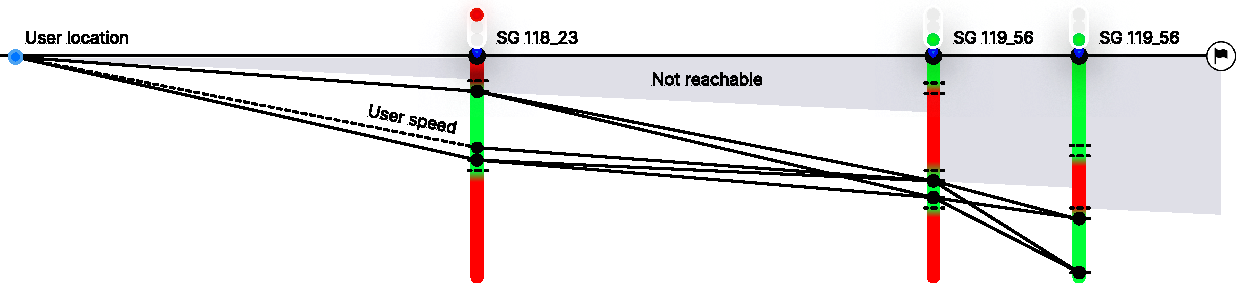
\includegraphics[width=\linewidth]{images/multi-segment-approach.pdf}
\caption{Initial idea of a graph alignment for multi-segment speed recommendation.}
\label{fig:multi-segment-approach}
\end{figure}

The concept of target speed recommendation can be thought further by incorporating the predictions of multiple consecutive traffic lights. For this purpose, a multi-segment speed advisory algorithm was conceived. The multi-segment approach aims to align the starting and ending points of green phases in a graph structure. By calculating the necessary acceleration and deceleration using a cost function, an approximation of the optimal trajectory could be efficiently determined using a pathfinding algorithm. 

In theory, this approach sounds very attractive, but it is not worth further investigating for cyclists due to the following limitations that were encountered during our preliminary real-world tests on a demo track in Dresden and the real-world deployment in Hamburg:

\begin{enumerate}
\item \textbf{Issue of speed fluctuations and oscillation around the target speed:} One problem encountered was the varying user speed measurements caused by inaccuracies in geolocation. As a result, the difference between the target speed and the user's actual speed fluctuated from second to second, leading to a perceived lack of responsiveness. Additionally, since the user location (together with its speed) is maximally sampled once per second, we experienced stuttering recommendations instead of a smooth and continuous experience. This often resulted in excessive over- or under-compensation to reach the target speed, leading to an overall poor user experience.
\item \textbf{Failure to consider acceleration inertia:} Another limitation was the failure to account for the user's inertia in the calculation process. The calculation assumed that the user could instantly adjust to the recommended speed. However, the longer it took to match the speed recommendation, the greater the discrepancy became. Consequently, we felt a constant need to chase the speed recommendation, which contributed to a sense of dissatisfaction.
\item \textbf{Explainability of prediction uncertainties:} Another challenge is displaying the prediction's uncertainty to users. Although it is possible to incorporate the prediction's uncertainty into the calculation process, this process happens in the background and is not clear to the user. For example, the speed advisory may overly slow down the user (focusing on a certainly green part of the prediction) when the traffic light becomes green much earlier in the real world. The user could interpret this intended behavior as an imprecise speed advisory.
\item \textbf{Consideration of user limits and capabilities:} The speed advisory algorithm has to make assumptions about the user's physical abilities to accelerate and decelerate in a specific scenario. This is a major drawback, as users could be impeded by traffic or physically unable to meet the recommendations, leading to disappointment when a recommended speed can't be achieved. Even more frustration can occur with a false speed advisory after having spent additional energy to follow the recommended speed. While factors like incline in the path, surface quality, or the type of bike chosen (e-bike vs. regular bike) could be partially used to model the user's capabilities, not all real-world aspects perceived by the user can be adequately captured.
\item \textbf{Conflict with user intentions:} When providing a target speed recommendation, the system decides a speed for the user. However, the user's intention may be to ride comfortably while feeling pressured by the app to speed up. In situations where there is ambiguity, with some users opting to speed up while others prefer to slow down, the speed recommendation effectively works against one of these groups. Hence, it is generally desirable to offer multiple target speeds to provide users with some freedom of choice.
\end{enumerate}
 
These observations culminate in the following conclusion: in the context of bike-GLOSA apps, smartphones cannot model the real-world situation more adequately than the cyclist himself. Thus, the smartphone will likely make a less proper target speed decision than the user, given the same traffic light prediction. Therefore, it is important to investigate speed advisory user interfaces that allow users to flexibly choose between green phases of the upcoming signal: projection methods.

\begin{figure}[htbp]
\centering
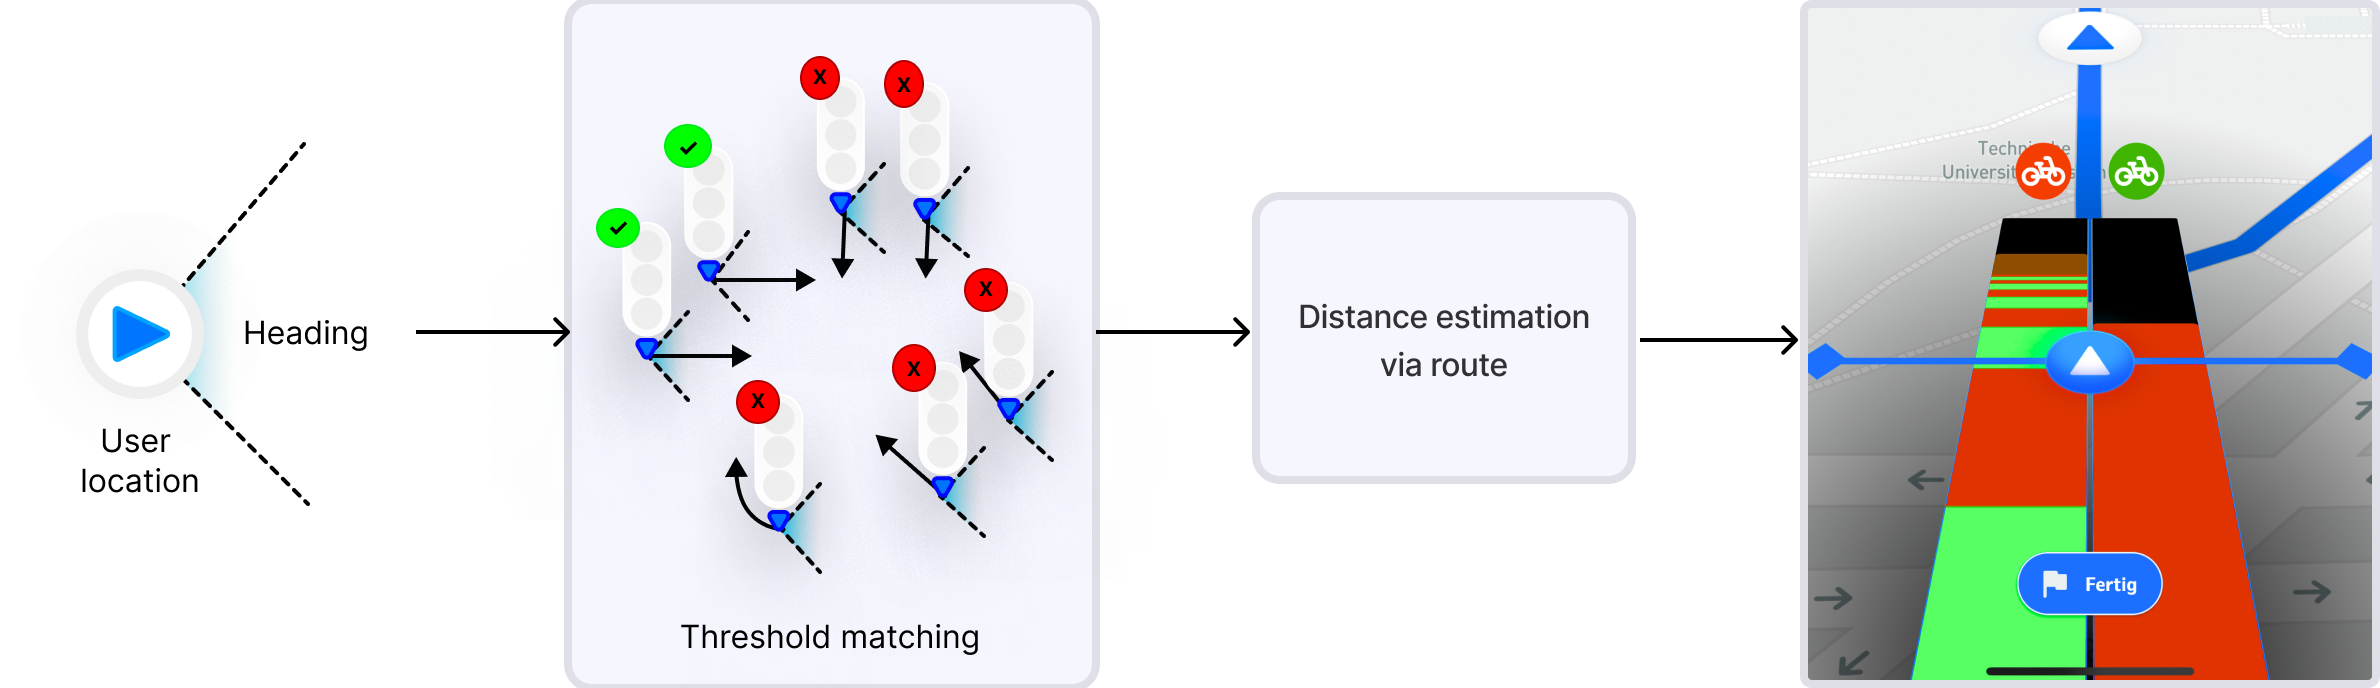
\includegraphics[width=\linewidth]{images/multi-lane-view.png}
\caption{Multi-lane matching and preliminary implementation of multi-lane speed recommendation.}
\label{fig:multi-lane-view}
\end{figure}

\paragraph{Multi-lane projection:} The multi-lane projection involves displaying multiple parallel lanes for upcoming traffic lights, with the prediction projected onto these virtual lanes. The user's location and speed are rendered above these lanes, allowing the user to slow down or speed up to move the prediction underneath. As the intersection comes closer, the lane's end (stop line) moves toward the user. This approach can be implemented by looking up all signals on intersections along the route which match the route's direction. The process is depicted in \Cref{fig:multi-lane-view}. Since all possible speeds are displayed, the user can flexibly choose between possible speeds. Furthermore, not a single traffic light is matched but multiple parallel signals at the intersection. This means that the user can select the appropriate signal, simplifying the traffic light matching process.

However, this approach comes with its own drawbacks. The main drawback is the visualization's readability while riding. With multiple parallel signals being displayed, users have to mentally correlate the shown lanes with the real-world situation ahead and process predictions for multiple parallel lanes simultaneously. Another challenge lies in moving the predicted traffic light colors intuitively towards the signal, resembling a flow in which the user can "jump on." A problem is choosing a suitable zoom scale for the prediction, such that users can differentiate when they will be "caught" or "run into" a red signal. Similar to the initial color-coded scale, users also have to get used to the direction of movement that they can induce when they speed up or slow down. Due to these concerns about the approach's usability and potential for distraction, another speed advisory user interface was tested: the speedometer projection.

\begin{figure}[htbp]
\centering
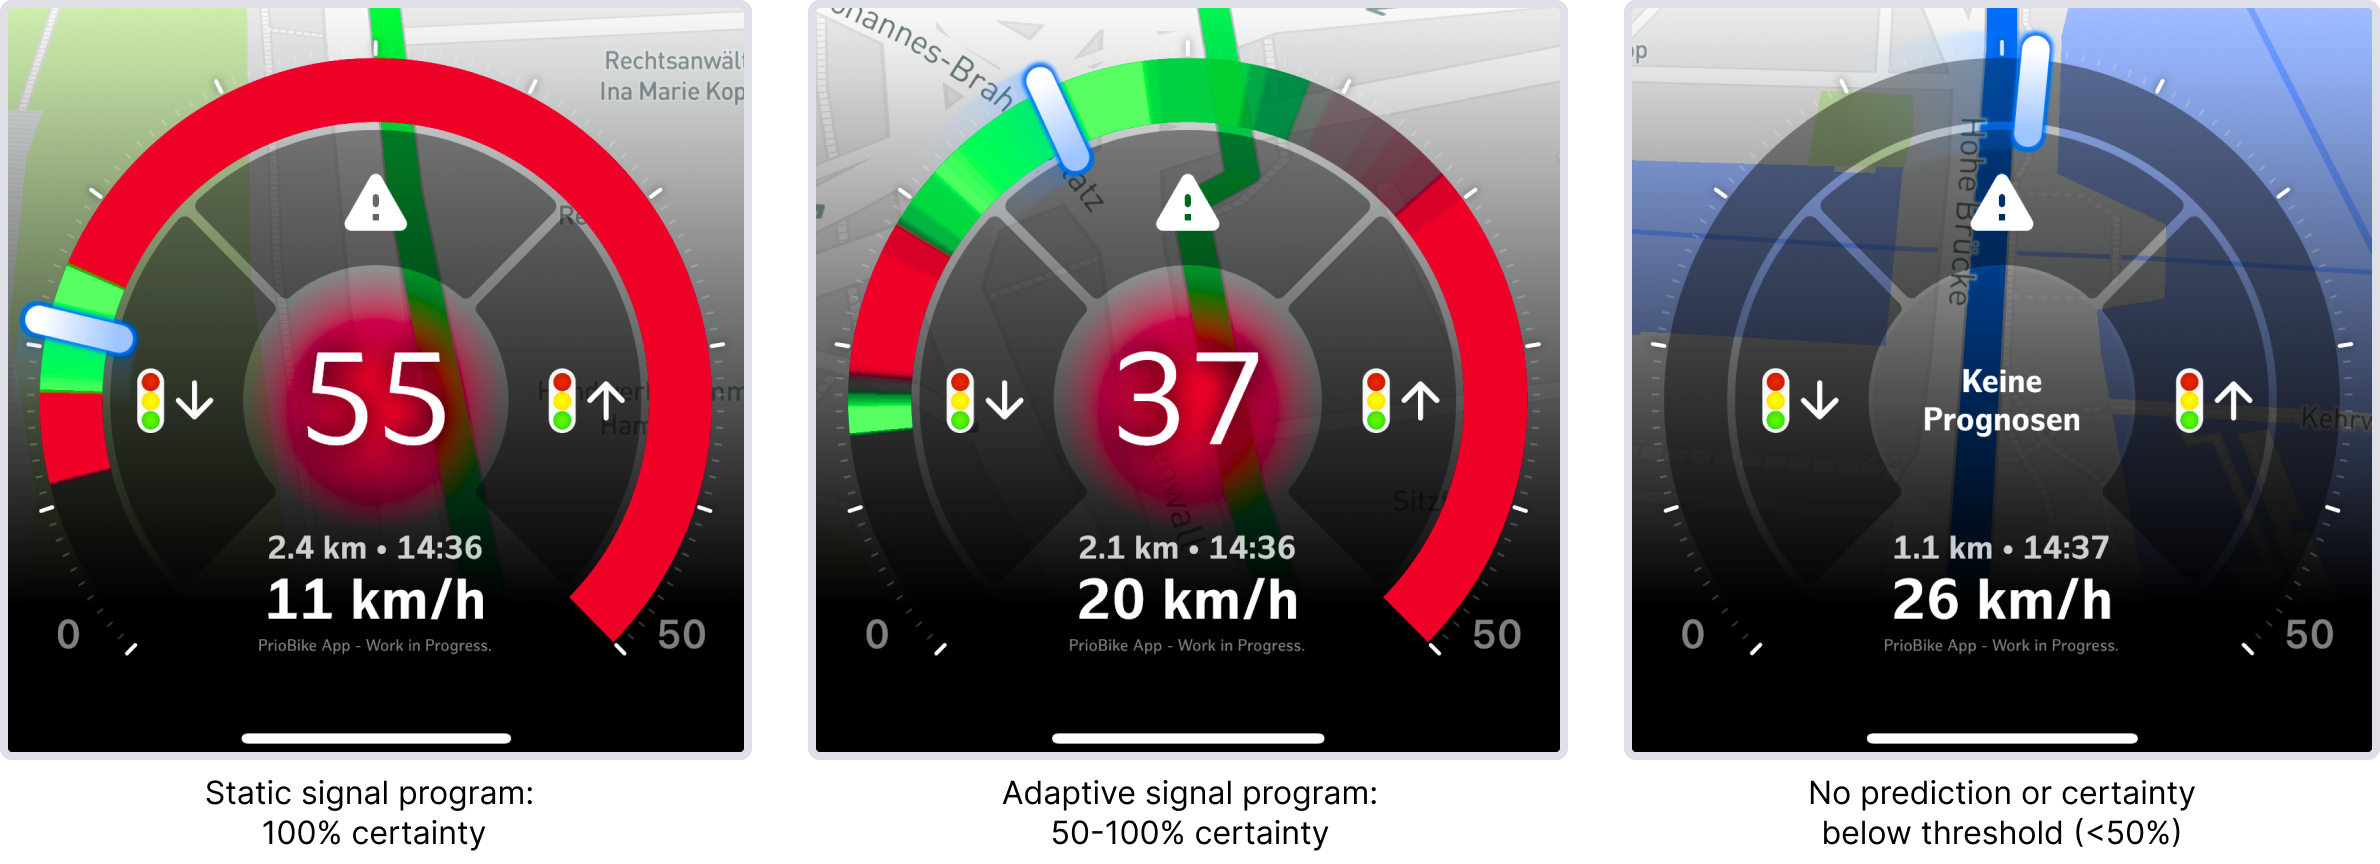
\includegraphics[width=\linewidth]{images/speedometer-adaptions.png}
\caption{Final speed recommendation concept and adaption mechanisms for varying prediction quality.}
\label{fig:speedometer-adaptions}
\end{figure}

\paragraph{Speedometer projection:} The final speed advisory visualization aims to integrate the strengths and mitigate the weaknesses of both previous approaches. It involves building a visualization around a speedometer, a widely recognized and, thus, probably more intuitive instrument for representing speed. Unlike the multi-lane visualization, only one relevant traffic light is selected by matching a sequence of upcoming traffic lights through the route geometry.

As confirmed preliminarily through initial field tests, this approach represents a noticeable improvement over both other approaches. The speedometer allows users to focus more on the real-world situation and occasionally glance at the display to determine if they are within a green window. Similar to the multi-lane visualization, the choice of target speed is entirely externalized to the user, and no speed recommendation algorithm is required. Hence, users have the freedom to select any target speed based on their current physical and contextual circumstances. This means that there is no potential for recommendation error and no need for advanced speed recommendation models. The only challenge that comes with this approach is precisely selecting the upcoming traffic light along the pathway. Since only one traffic light (instead of multiple parallel signals) is focused, the traffic light selection process has to be much more advanced.

To address prediction uncertainties, the speedometer incorporates a mapping of these uncertainties by adjusting the opacity of the green or red colors. This adaption is also highlighted in \Cref{fig:speedometer-adaptions}, and conveys certain and uncertain parts of the prediction to the user. Although this opacity mapping is also possible with the multi-lane visualization, the speedometer's prediction arc utilizes the available screen space much more efficiently, which makes the prediction uncertainties more easily conceivable. To avoid users adapting to a poor speed recommendation, the speed advisory is only displayed if the prediction quality is above 50\%. Additionally, to compensate for fluctuations in the measured GNSS speed, a smooth animation is applied to the speedometer needle. On top, a time-to-green (or time-to-red) countdown has been included at the center of the speedometer. This countdown is hidden either 5 seconds before the traffic light switches or if the prediction quality is too low, avoiding jump starts or inadvertently running a red light. This idea was adopted from other time-to-green displays observed in Dresden that are mounted onto a traffic light and hide their countdown a few seconds before switching as well.

To conclude this section, three identified visualization methods have been investigated and thoroughly tested. Observed disadvantages of other visualizations ultimately lead to the conclusion that the speedometer visualization is the best possible speed advisory visualization for cyclists. Thus, this design is selected as the final approach.

\subsection{Orientation and Wayfinding}

\paragraph{Camera Controller for Improved Traffic Light Visibility:} The main purposes of the map view are to display the user's current route and to show which signals are along the way. In this way, the user sees if a traffic light is connected to the TLD system and for which traffic light the current speed advisory is displayed. Initially, a camera was implemented that strictly follows the user's position and heading at a fixed height. However, often, the currently selected traffic light was out of view, or the camera was too far away at an intersection or a specific turn. Thus, the map's camera has to dynamically adjust its height depending on the situation, but without being distractive.

Furthermore, there would be occasions when road bends were between the user and the signal. In this case, since the heading of the user was strictly followed, the route would curve away from the map view, making it hard to see the upcoming signal. Through studying other navigation apps, it was observed that Apple Maps employs a slight rotation of the map to provide users with a better overview of upcoming turns. A screenshot of this behavior is highlighted in \Cref{fig:camera-controller}. This behavior, in addition to automated zooming, was adopted to improve the overall usability and self-sustainedness of the map view.

\begin{figure}[htbp]
\centering
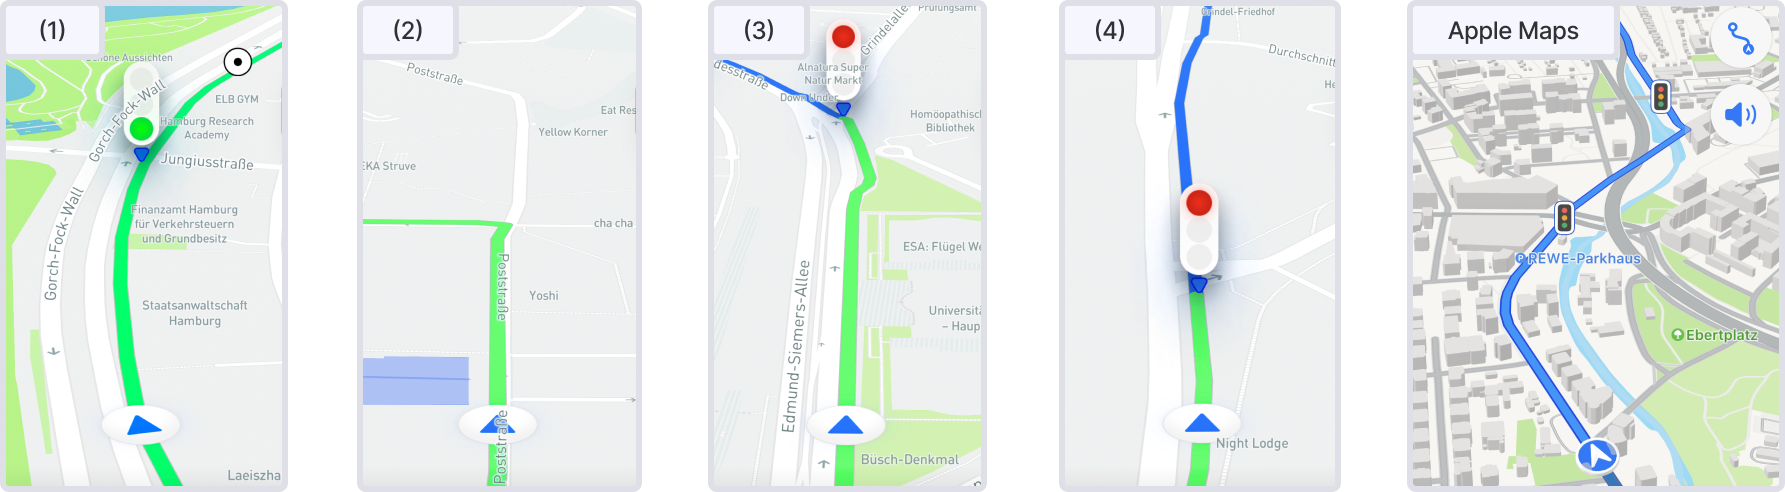
\includegraphics[width=\linewidth]{images/camera-controller-1.png}
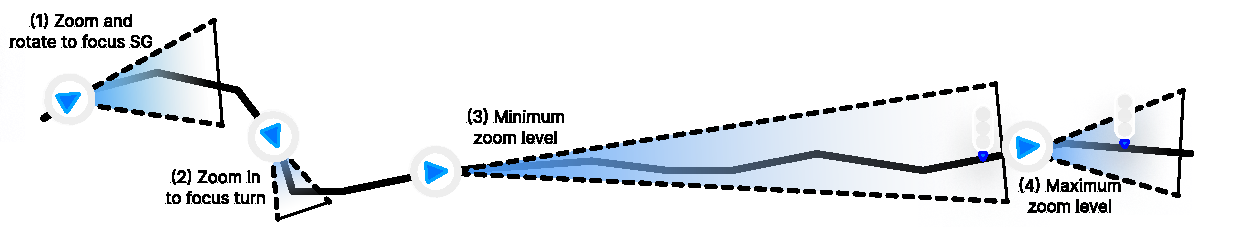
\includegraphics[width=\linewidth]{images/camera-controller-2.pdf}
\caption{Dynamic camera adaption in different scenarios.}
\label{fig:camera-controller}
\end{figure}

During a ride, the app continuously checks if the user is approaching a traffic light by examining the route segments from the user's location. A turn is detected when a route segment is found that deviates at least 15° from the user's measured heading. As the user approaches a turn or traffic signal, the camera automatically zooms in to focus on the intersection, making it easier for users to locate a path entry or identify a corresponding signal. Additionally, the camera rotates slightly (up to a maximum of 20°) away from the user to ensure that the traffic lights remain within the view frustum. These threshold values have been determined empirically through extensive real-world testing. To prevent excessive zooming, the camera operates within specified maximum and minimum zoom levels, avoiding zooming too far out or too far in.

There are several factors that can influence a cyclist's route choice. For instance, cyclists may opt for a slightly less optimal route if it offers better surface quality. One approach is to incorporate this information directly into the routing profile to ensure that each user receives an enhanced routing decision. This is already supported by GraphHopper's routing profiles, defining different speeds for each \texttt{vehicle} depending on the road segments' metadata. However, it is important to acknowledge that GraphHopper's routing profiles are mathematical models that make complex assumptions and, therefore, cannot always produce the ideal route. From the user's perspective, it can often be hard to understand a particular route choice without any further explanation as to why specific paths have been chosen. This is a problem for users, especially if they are familiar with the area and already have a preferred route. Thus, to build trust in the routing, it is vital to provide additional route details to allow users to make informed routing decisions.

\begin{figure}[htbp]
\centering
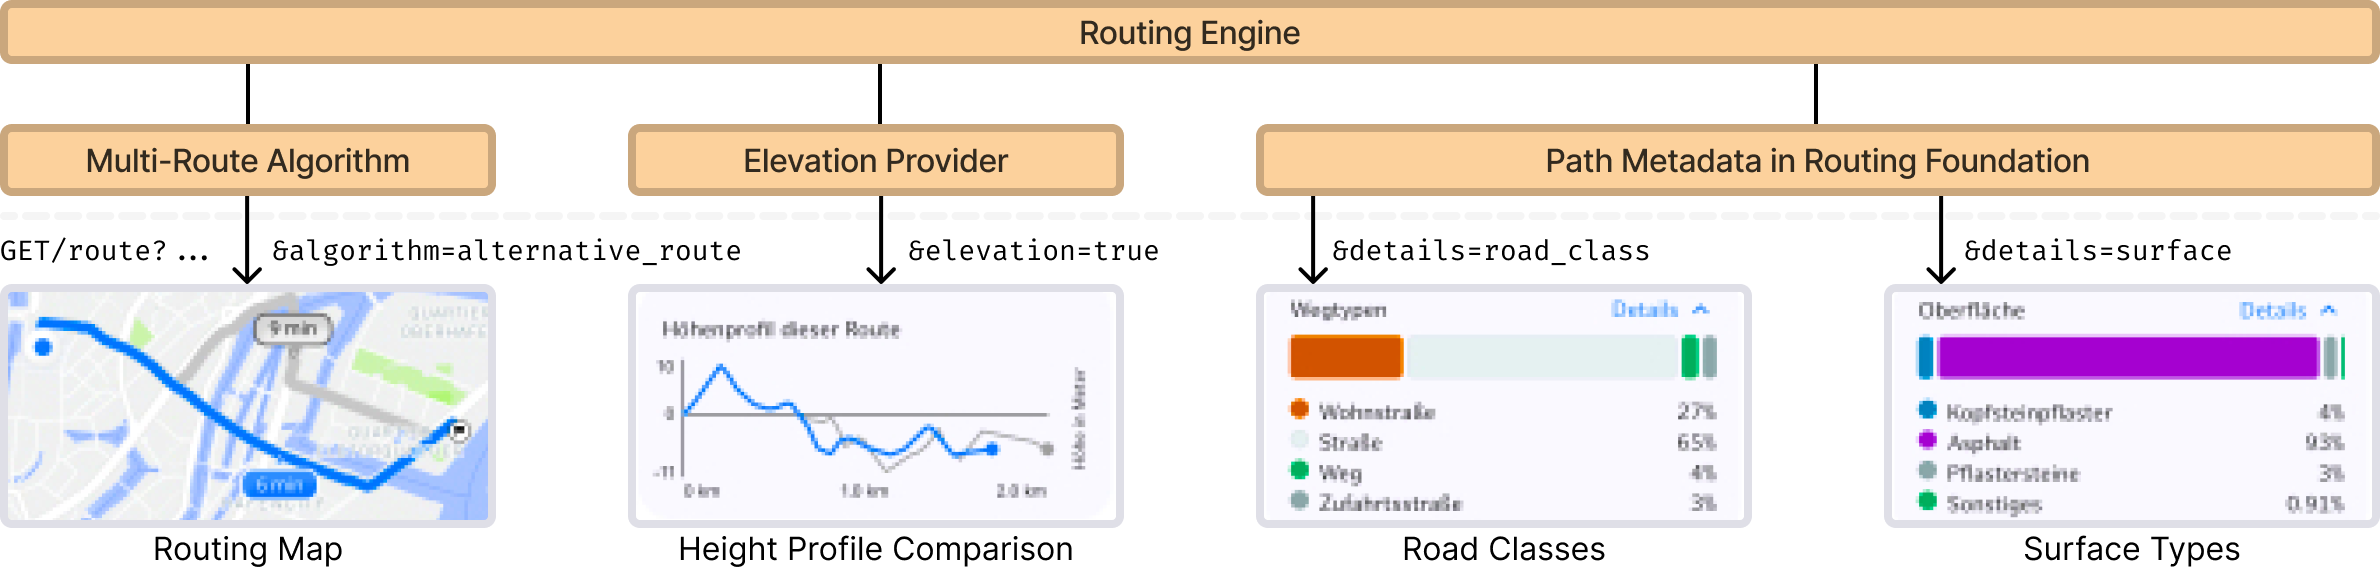
\includegraphics[width=\linewidth]{images/graphhopper-data-flow.png}
\caption{Visualization and fetching of alternative routes and other metadata.}
\label{fig:graphhopper-data-flow}
\end{figure}

To support users and make the route decision process more transparent, additional information is provided about the surface type, elevation, and road classes along the route so that the user can form their own opinions about the suitability of the chosen route. All of this information is fetched from the routing engine, as highlighted in \Cref{fig:graphhopper-data-flow}.

\paragraph{Traffic Flow Prediction:} In addition to the path's surface information and inclination, the traffic density may also have a large impact on the ride's perceived comfortability and safety. Google Maps has addressed this problem by showing users a predicted traffic density for the following hours. The foundation for these calculations is floating data: "To determine popular times, wait times, and visit duration, Google uses aggregated and anonymized data from users who have opted in to Google Location History."\footnote{Source: \url{https://support.google.com/maps/answer/11323117?hl=en}} To adopt a similar solution without relying on a large user base, we can make use of open floating car data from the company INRIX provided through the TraffGo Road GmbH (see \Cref{fig:traffic-density-prediction}). The publicly available dataset "Verkehrslage Hamburg" is updated every five minutes and contains a current traffic density status for each path in Hamburg: free-flow, dense, heavy, and congested traffic. Based on this data, a traffic flow prediction for Hamburg is designed.

\begin{figure}[htbp]
\centering
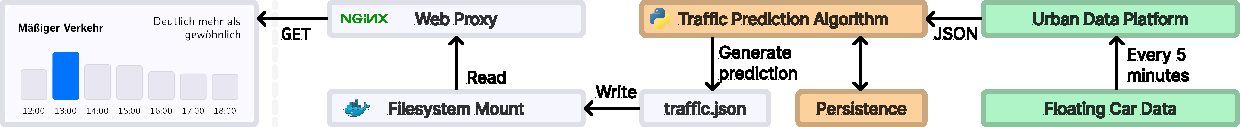
\includegraphics[width=\linewidth]{images/traffic-density-prediction.pdf}
\caption{Data flow of traffic density prediction toward the app.}
\label{fig:traffic-density-prediction}
\end{figure}

To obtain an overall traffic flow factor $\text{Flow}$ for Hamburg, the following algorithm is designed. Let $P$ be the set of all paths in the "Verkehrslage Hamburg" dataset, and $n$ be the number of paths in $P$. For each path $i$ in $P$, let:

\begin{itemize}
    \item $L_i$ be the length of path $i$.
    \item $W_i$ be the weight associated with path $i$: congested $\rightarrow 0$, heavy $\rightarrow 1/3$, dense $\rightarrow 2/3$, and free-flow $\rightarrow 1$
\end{itemize}

The total length $L_\text{network}$ of all paths is given by: $L_\text{network} = \sum_{i \in P} L_i$. Then, the score $S_i$ of each path in relation to the complete network is calculated as $S_i = \frac{L_i}{L_\text{network}} \times W_i$. Now, the resulting $\text{Flow}$ is the sum of all scores: $\text{Flow} = \sum_{i \in P} S_i$. 

The value of $\text{Flow}$ is always in $[0, 1]$, where 0 indicates complete congestion of all roads, and 1 indicates free flow on all roads. In Hamburg, typical values lie within 0.94 (maximum traffic) and 0.99 (minimum traffic). This empirically defined boundary defines the min-max scaling of the user interface as highlighted in \Cref{fig:traffic-density-prediction}. This means that values of 0.94 will be displayed as a full-height bar, and 0.99 will be displayed as a bar with 0 height. 

To predict the traffic flow, a history is persisted for every hour and weekday. Now, each hour is predicted through the arithmetic mean of all previously recorded hours on the same weekday. If the service starts freshly and has no recording of the same weekday, the hourly average is calculated by all other available weekdays. The generated prediction contains the current measured $\text{Flow}$ value, as well as predicted values for the previous, current, and next 5 hours. The continuously updated JSON data is served through a web proxy to the mobile app.


\begin{figure}[htbp]
\centering
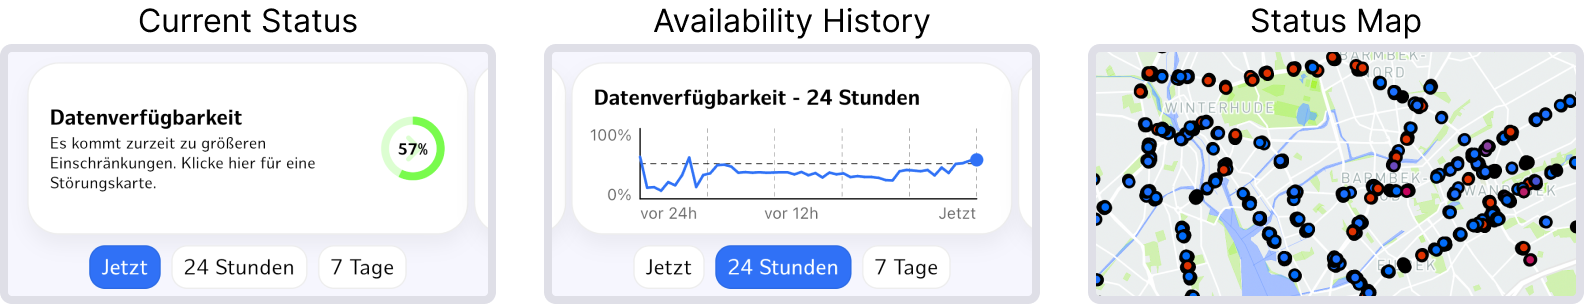
\includegraphics[width=\linewidth]{images/home-view-prediction-quality.png}
\caption{Prediction quality visualized in the GLOSA app for enhanced explainability.}
\label{fig:home-view-prediction-quality}
\end{figure}

Not all traffic lights in Hamburg are available for prediction. Those who are available may occasionally lose data, which error detection can partially address. Another important factor, however, is the user's perspective on the data availability. Since a degraded prediction availability will also negatively impact usability, some ideas must be found that mitigate potential disappointments on the user side. One idea implemented in the GLOSA app is increasing the explainability of the prediction system. The existing monitoring infrastructure is extended such that users can also access information about the current availability. Through the app, users can inform themselves about the current percentage of available predictions and the spatial distribution of good and bad predictions on the map. The resulting user interface shown in \Cref{fig:home-view-prediction-quality} is intended to allow users to identify faults at an early stage and then switch to an alternative app, avoiding frustration caused by missing or incorrect predictions.

\paragraph{Prediction Availability:} As discussed previously, predictions and, therefore, speed recommendations are not available for all intersections in Hamburg. Furthermore, traffic-adaptive signals or data outages may lead to low-quality or missing predictions. Therefore, it is crucial for the user to see along which route segments a speed advisory can be expected. To communicate the prediction availability to users, the route is highlighted in green wherever a "green wave" can be expected.

\begin{figure}[htbp]
\centering
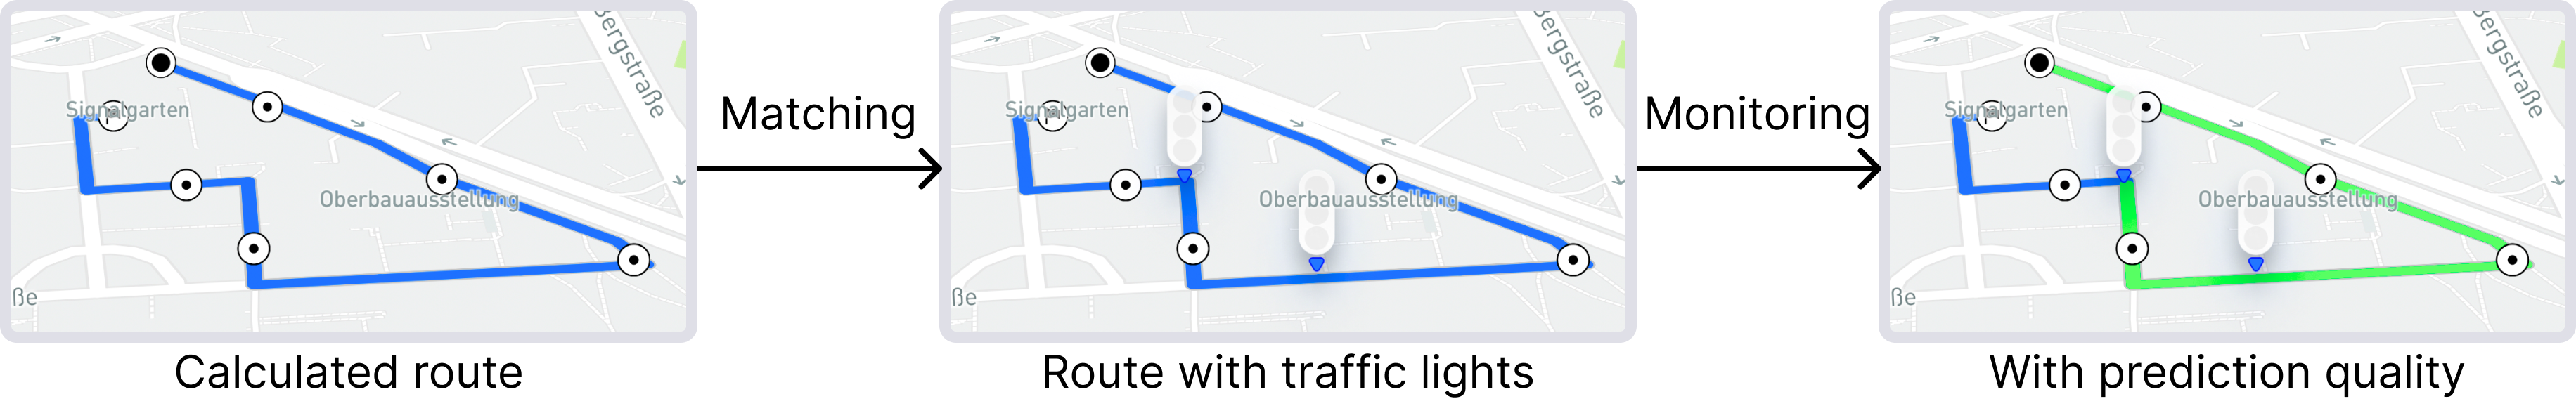
\includegraphics[width=\linewidth]{images/routing-process-quality-mapping.png}
\caption{Visualization of traffic light groups and prediction quality along the calculated route.}
\label{fig:routing-process-quality-mapping}
\end{figure}

To match the prediction qualities onto the route, two steps illustrated in \Cref{fig:routing-process-quality-mapping} are performed: First, the signals are matched along the route. Afterward, the obtained traffic light IDs along the route are utilized to fetch and map the prediction qualities generated by the prediction monitor. Finally, the route is colorized with respect to the prediction quality. No prediction means the route is not colored green. A prediction with less than 50\% quality is also not displayed as green since no speed advisory is activated. Upwards, the color is interpolated between the default route color (50\% quality) and green (100\% quality). 

\paragraph{Bike-Specific Points of Interest:} Routes can only be calculated if the users define their destination or multiple waypoints. Thus, users have to be given the option to look up places through the app. One option is to pinpoint a location on the in-app map. Here, it is vital to provide more information than just the base map layer. For example, Google Maps highlights specific places, such as busy areas, to improve the map's informativeness. In the designed solution, the focus lies on bike-specific points of interest, such as repair shops, parking spots, rental stations, and air pumps. A traffic layer is also provided, which indicates congested roads. Velo routes and static bike green waves (at 18 km/h) are also displayed to highlight public initiatives to make cycling more attractive. Furthermore, construction sites and accident hotspots can be marked on the map, providing enhanced awareness of potentially dangerous spots.

\begin{figure}[htbp]
\centering
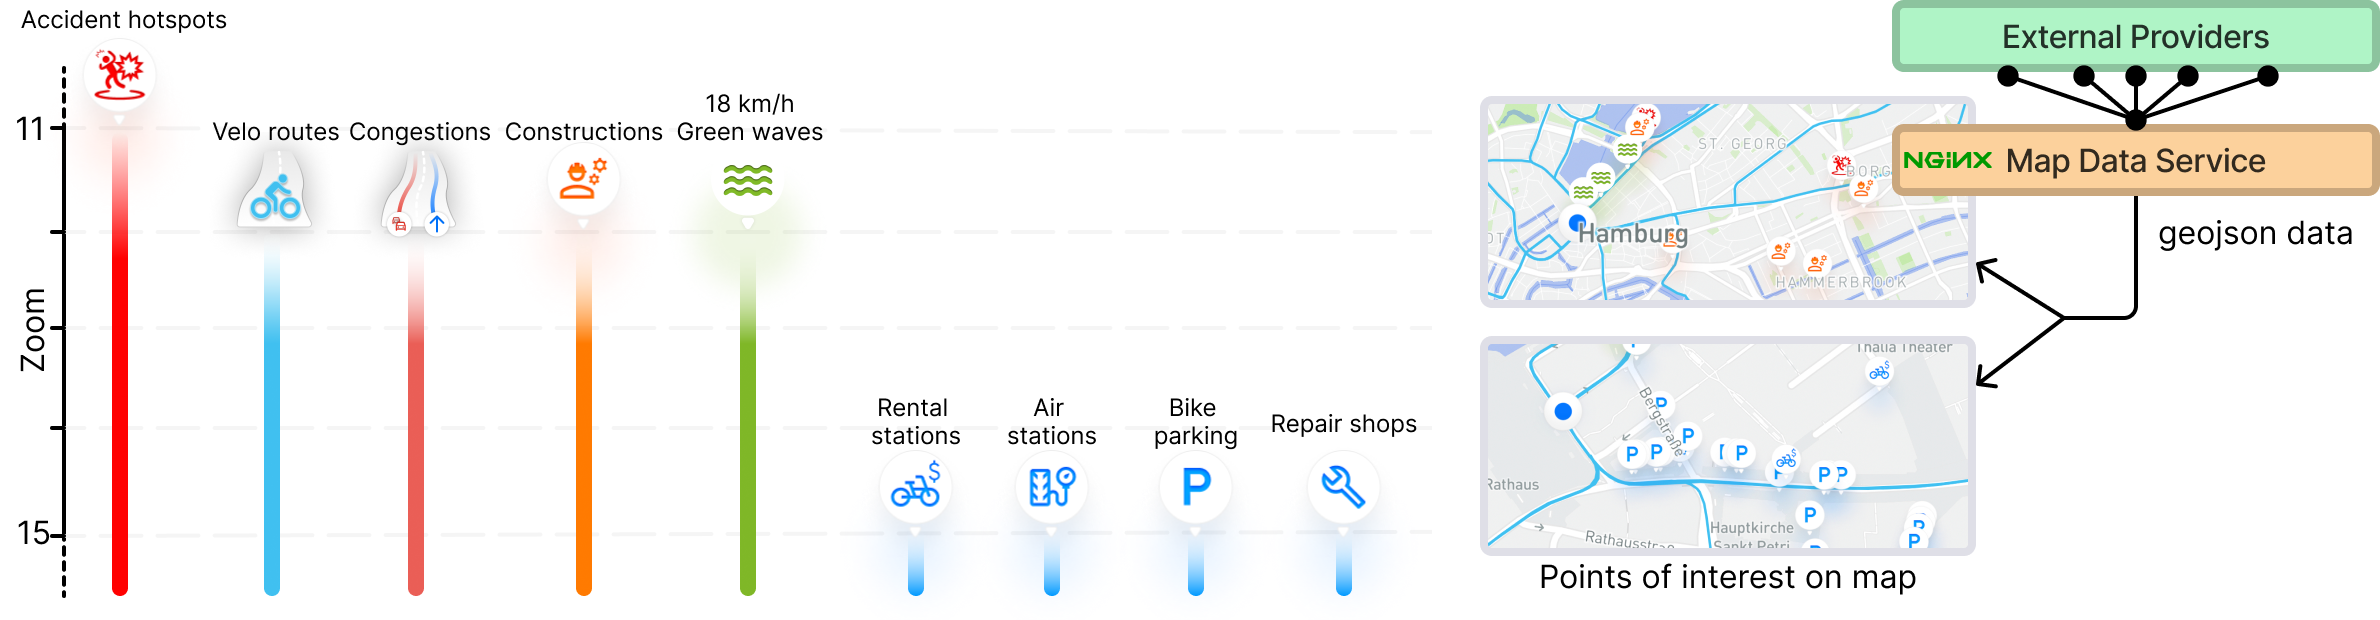
\includegraphics[width=\linewidth]{images/points-of-interest.png}
\caption{Hierarchical fade-in schema for map layers.}
\label{fig:points-of-interest}
\end{figure}

With this number of different points of interest, the risk of cluttering the map is high. Especially bike parking spots are present in large numbers all over the city. To circumvent this problem, the draw distances of map layers are ordered using a hierarchical schema. This hierarchical schema is highlighted in \Cref{fig:points-of-interest}. Points of interest that may potentially impact the cyclist's route choice are visible when zoomed out, while points of interest that are typically more relevant in proximity to the user are only displayed once zoomed in. Accident hotspots represent a special role and are displayed from farther out to further emphasize them on the map.

\paragraph{Accident hotspot extraction:} Under supervision, Markus Wieland \cite{wieland_2022} designed an accident hotspot extraction procedure based on the Unfallatlas\footnote{\url{https://unfallatlas.statistikportal.de/}} dataset. Bike accidents are extracted from the dataset and clustered, adding up the total number of bike accidents for each cluster. The resulting cluster accident counts are subjected to a threshold and, if exceeding this threshold, marked as accident hotspots.

\paragraph{Geocoding:} To create human-readable waypoints and search for places, a geocoding service is required to convert textual input into geospatial coordinates (geocoding). Likewise, when the user taps on the map to add a new waypoint, a similar service is needed to translate the coordinates into an address for the route planning view (reverse geocoding).

\begin{figure}[htbp]
\centering
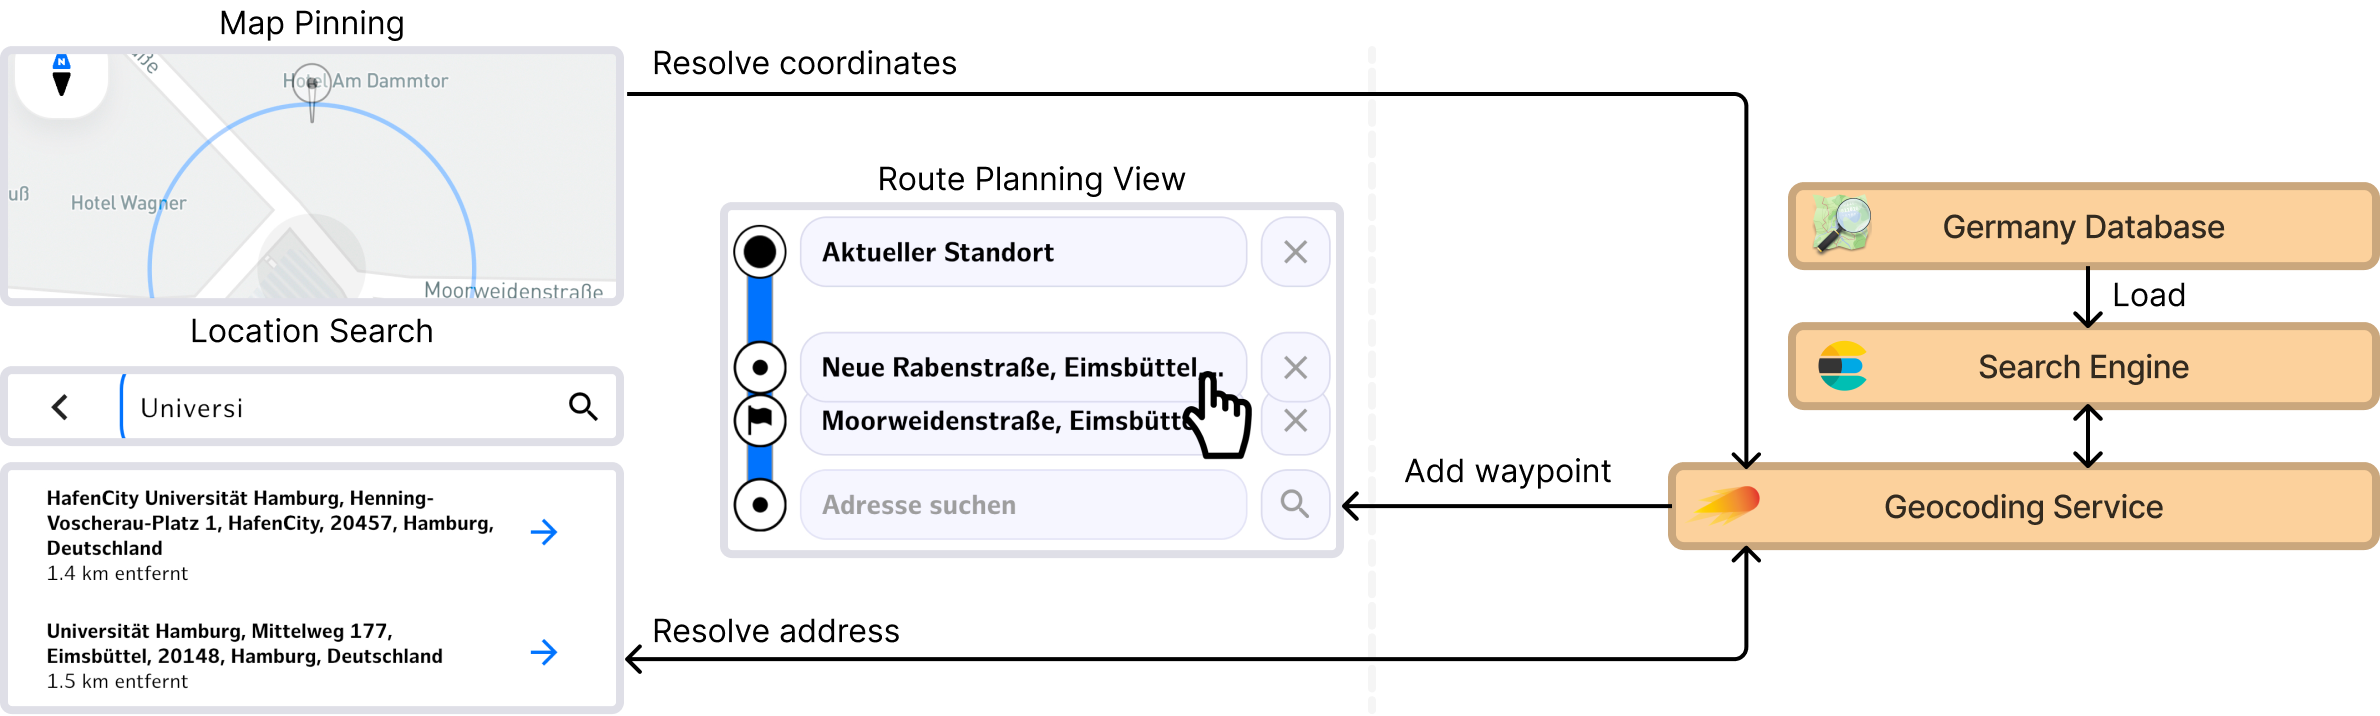
\includegraphics[width=\linewidth]{images/routing-view-geocoding.png}
\caption{(Reverse) geocoding via Photon for location search and map pinning.}
\label{fig:routing-view-geocoding}
\end{figure}

Initially, Nominatim was chosen as a geocoding service based on OpenStreetMap. However, the solution has shown limitations when it comes to supporting partial queries, such as searching for "University" using "Univers", and its response time was perceived as too slow (often more than 2 seconds) during preliminary tests. Therefore, as shown in \Cref{fig:routing-view-geocoding}, the decision was made to switch to Photon (by Komoot) as an alternative open-source solution that supports partial queries and provides faster query execution based on an ElasticSearch database.

\subsection{Final Application Architecture and Design}

\begin{figure}[htbp]
\caption{Final application infrastructure.}\label{fig:architecture}
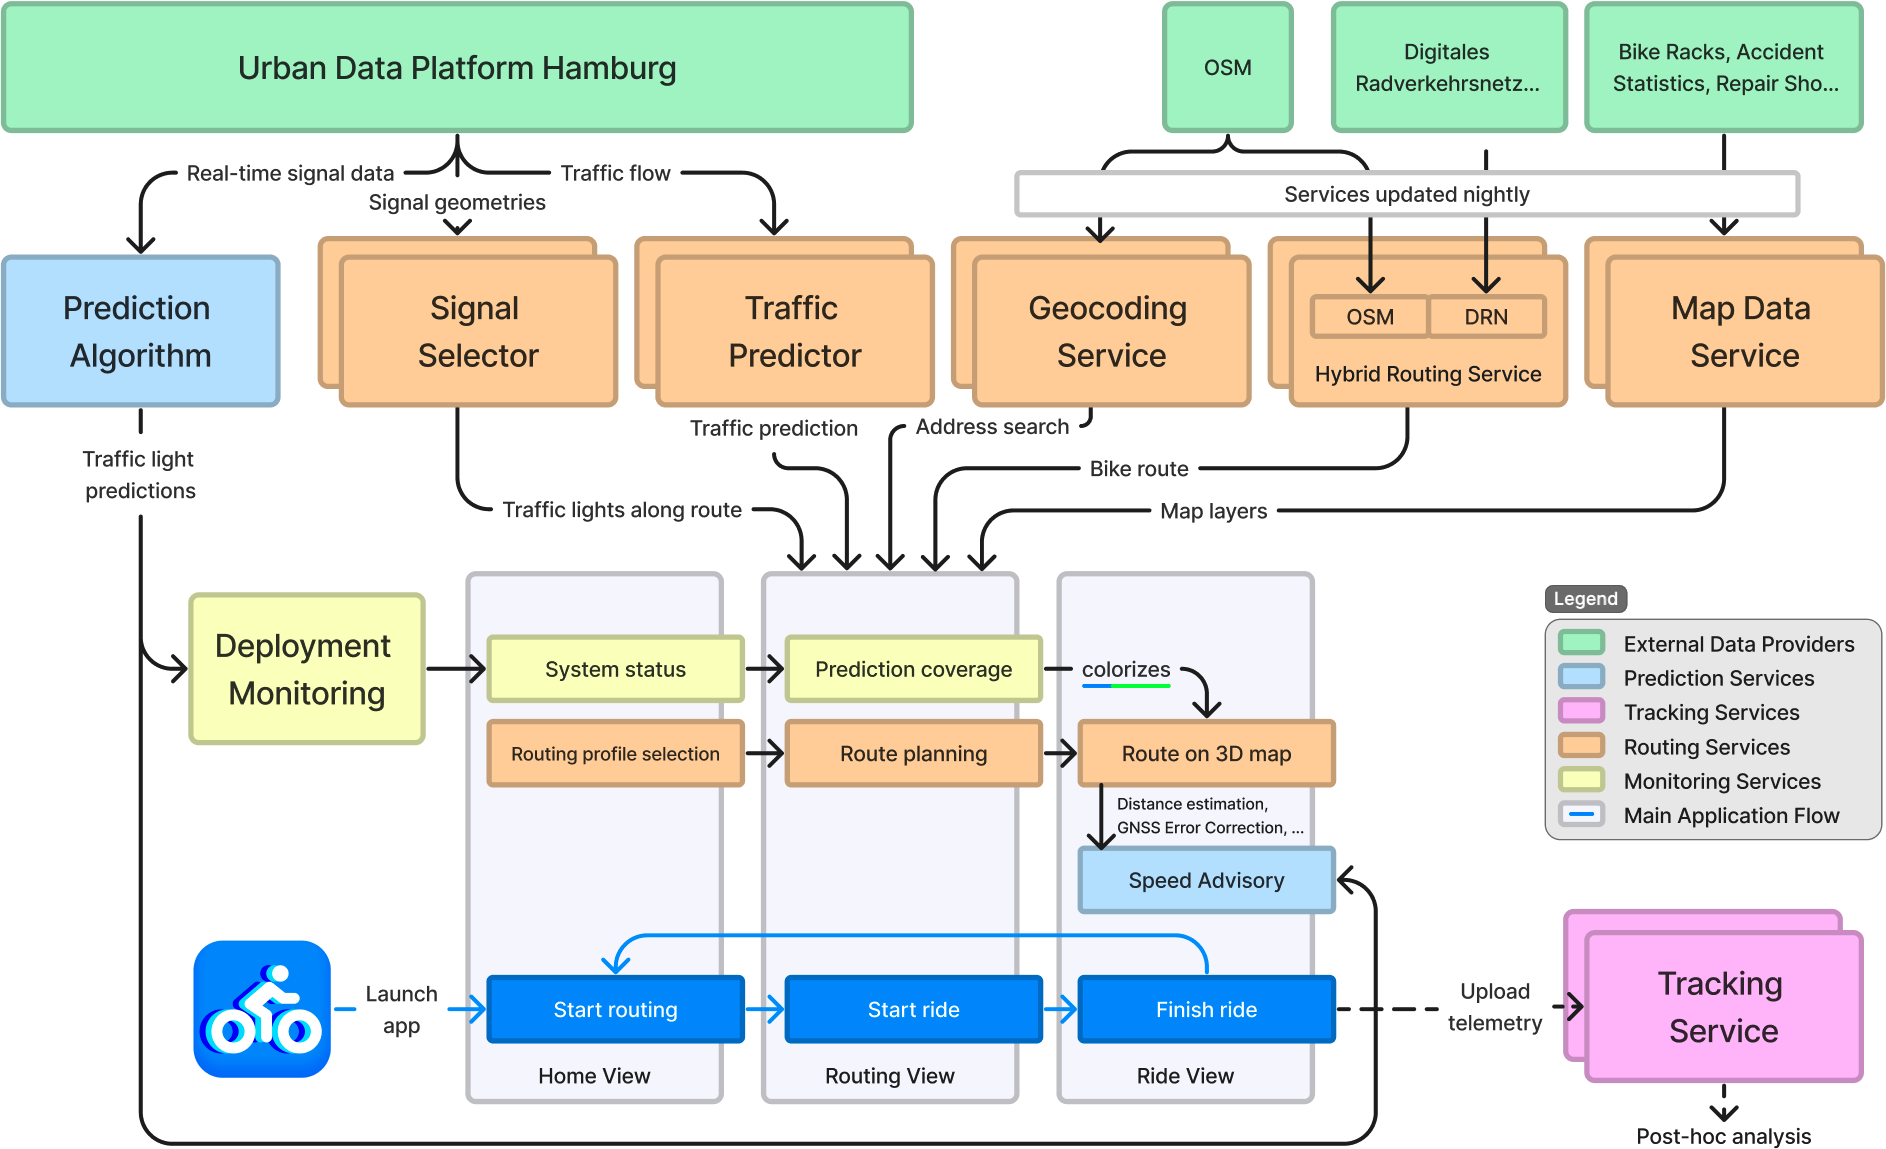
\includegraphics[width=\linewidth]{images/architecture.png}
\end{figure}

\Cref{fig:architecture} highlights the final service infrastructure that combines the developed solutions. The first key solution to make a bike-GLOSA app practical in a real-world urban environment is handling massive amounts of traffic light data. A prediction infrastructure (blue) is proposed that maximizes data ingress stability and self-monitors prediction qualities and availability. These metrics are used within the mobile application to adapt the speed advisory user interface and inform users about data outages.

A speed advisory user interface (the Ride View) is designed that utilizes the speedometer projection to give users a free choice of the desired speed. Uncertainties in the prediction are visualized to enhance the speed advisory's trustworthiness. To make the speed advisory practical, a user-defined route is used for distance-to-signal estimation, traffic light matching, battery-efficient GNSS error correction, and a camera controller for improved traffic light visibility. Combining the speed advisory system with a navigation solution is another key idea to enable these methods and make the mobile application useful in the absence of traffic light predictions.

To deliver bike navigation, a routing infrastructure (orange) is implemented that provides personalized, accurate, and metadata-enhanced bike routing. Once waypoints are found using the Geocoding Service and the Map Data Service that delivers bike-specific points of interest, an accurate bike route is calculated through the developed DRN approach. Route metadata and the predicted traffic situation are visualized to allow for a more informed routing decision. Generated routes are marked green at spots where users can expect a speed advisory. The routing material's actuality is ensured through an automated update CI/CD pipeline. 

The final key solution that connects the speed advisory to the routing is route-based traffic light matching. Multiple approaches were tested, coming to a final machine-learning-based method that compares geometric features between the traffic light geometries and the route geometry to decide which sequence of signals will be passed along the trajectory. To avoid giving a speed advisory for the wrong intersection, unconnected intersections are detected and also matched along the route.

Finally, a tracking service is implemented that obtains ride statistics from users. The collected telemetry data is used to conduct post-hoc analyses on the actual impact of bike-GLOSA on ride behavior. \Cref{ch:results} will focus on the analysis of this data.

\begin{figure}[htbp]
\caption{The PrioBike app's main view flow.}\label{fig:app}
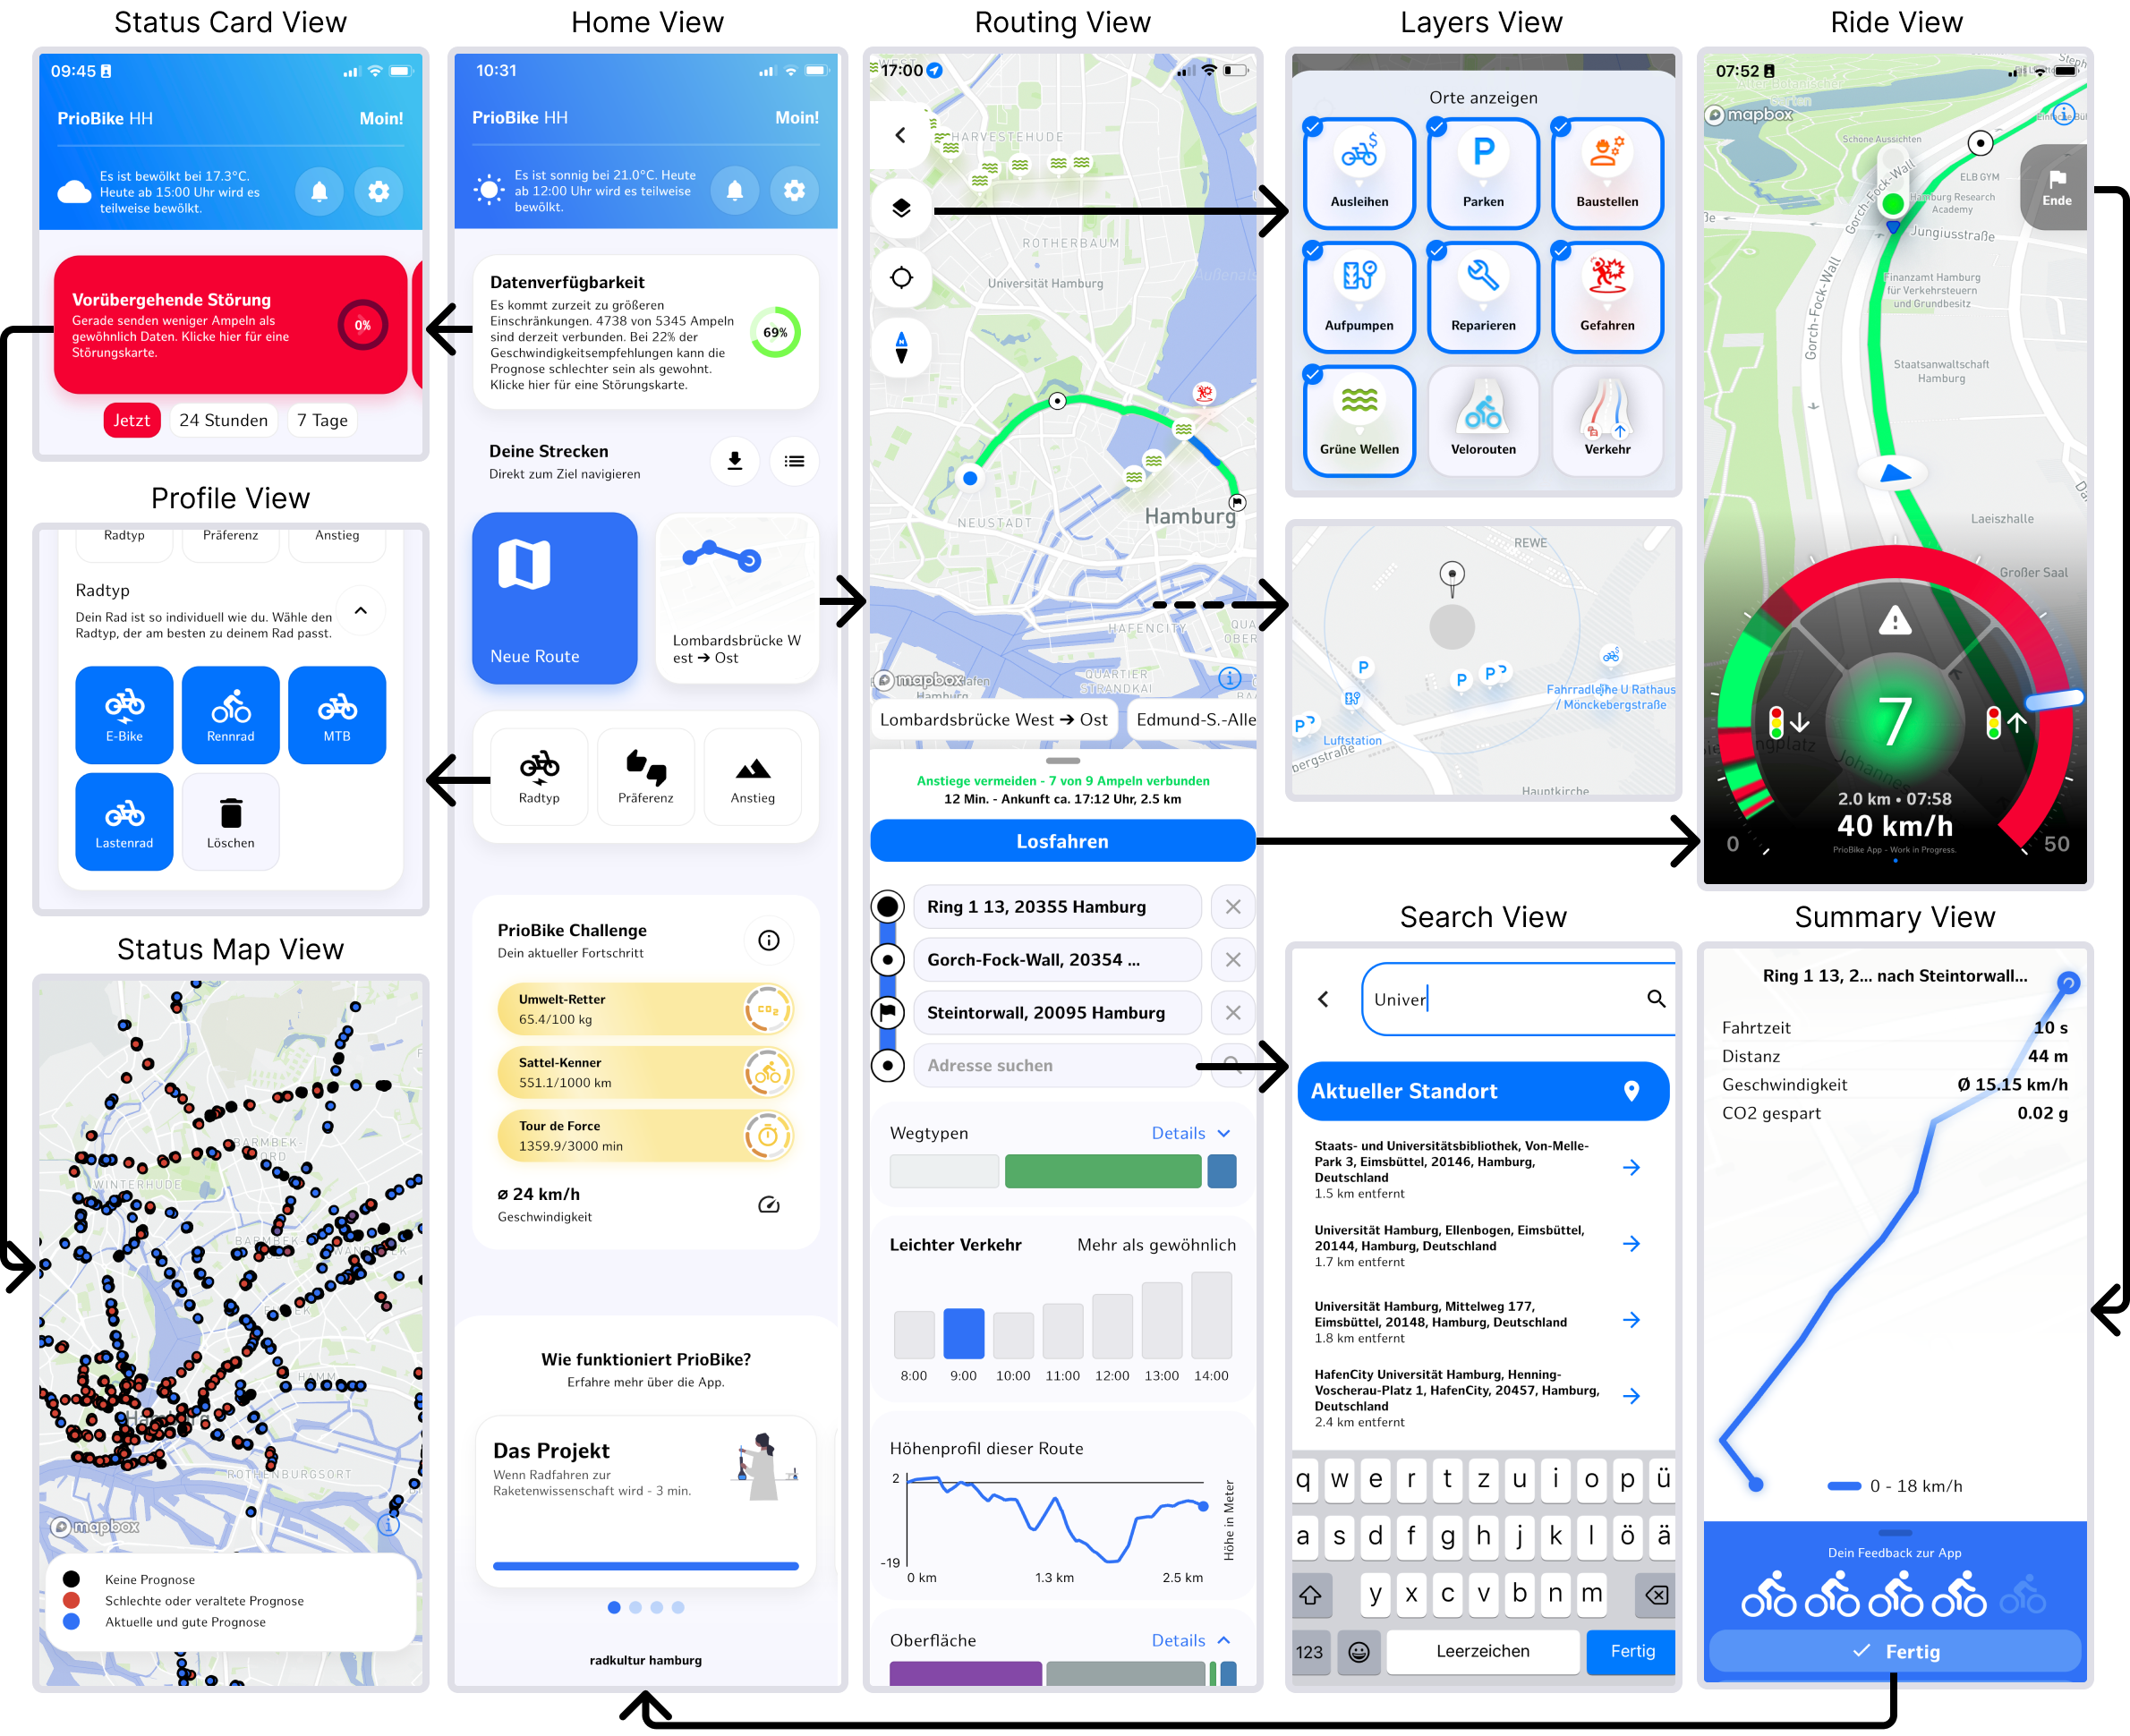
\includegraphics[width=\linewidth]{images/app.png}
\end{figure}

What's visible to the user is an application similar to other navigation apps like Google Maps or Komoot, with added speed advisory functionality. \Cref{fig:app} shows how the designed user interface components are combined into a cohesive application flow concept. From the Home view, which allows users to inform themselves about the current prediction status, users can personalize their routing profile and open the Routing view. This view provides the described route planning functionality. Finally, users can start a ride to obtain the discussed speed advisory. A summary is given after the ride, together with the option to rate the application experience. This rating, together with the collected ride and prediction data, is sent to the tracking service in an optionally offloaded upload routine.

The final application is distributed to real-world test users in Hamburg, who can freely use the app throughout the city to provide realistic experimental circumstances for the urban cycling setting. Based on the collected data, surveys, and other experiments, the next goal is to determine the impacts of such a solution. These aspects will be discussed in the following chapter.

\section{Results}

\subsection{Usability}

- SUS Score
- Interaction during ride
- General user feedback

\subsection{Impact on Approach Speed, Stop Time, and Energy Expenditure}

\begin{figure}[t]
\caption{T.}\label{fig:}
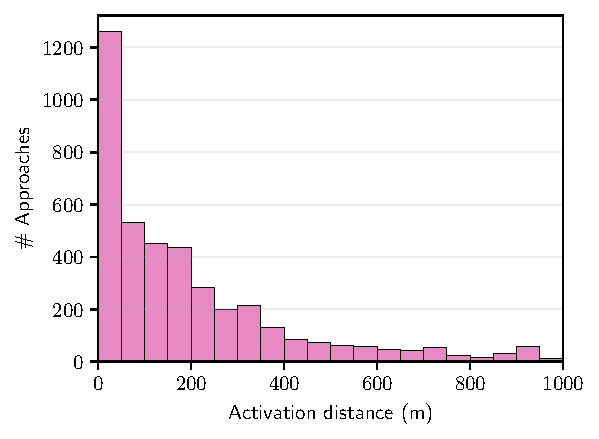
\includegraphics[width=\linewidth]{images/impacts-activation-distances.pdf}
\end{figure}

\begin{figure}[t]
\caption{T.}\label{fig:}
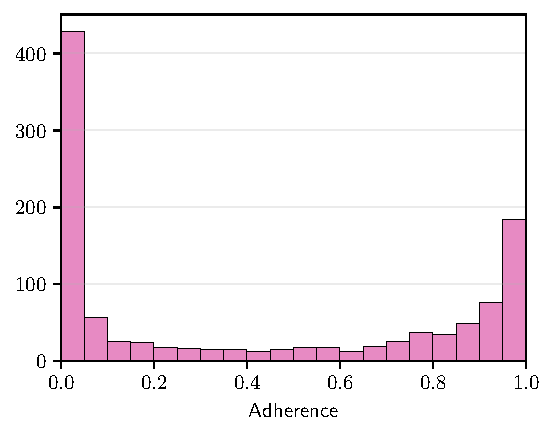
\includegraphics[width=\linewidth]{images/impacts-adherence.pdf}
\end{figure}

\begin{figure}[t]
\caption{T.}\label{fig:}
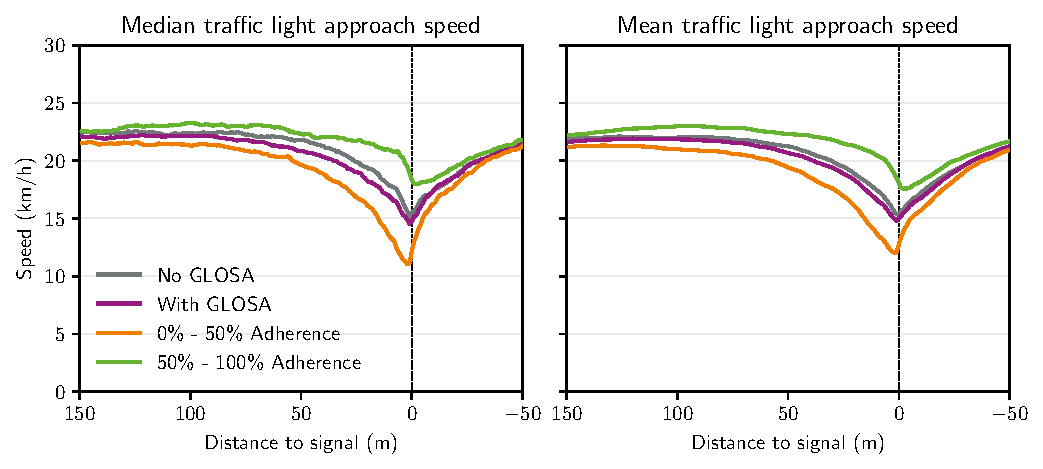
\includegraphics[width=\linewidth]{images/impacts-approach-speed.pdf}
\end{figure}

\begin{figure}[t]
\caption{T.}\label{fig:}
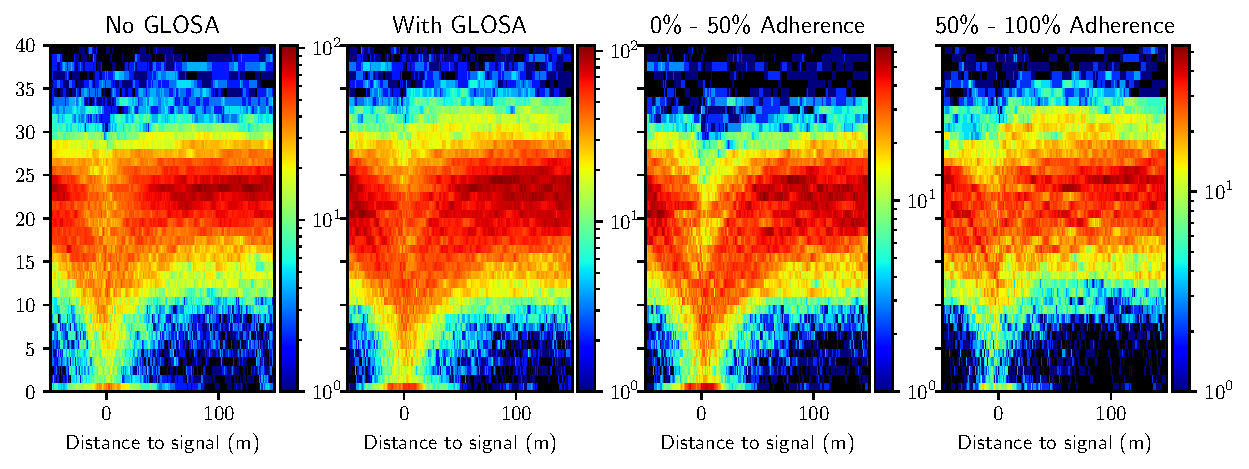
\includegraphics[width=\linewidth]{images/impacts-approach-speed-heatmap.pdf}
\end{figure}

\begin{figure}[t]
\caption{T.}\label{fig:}
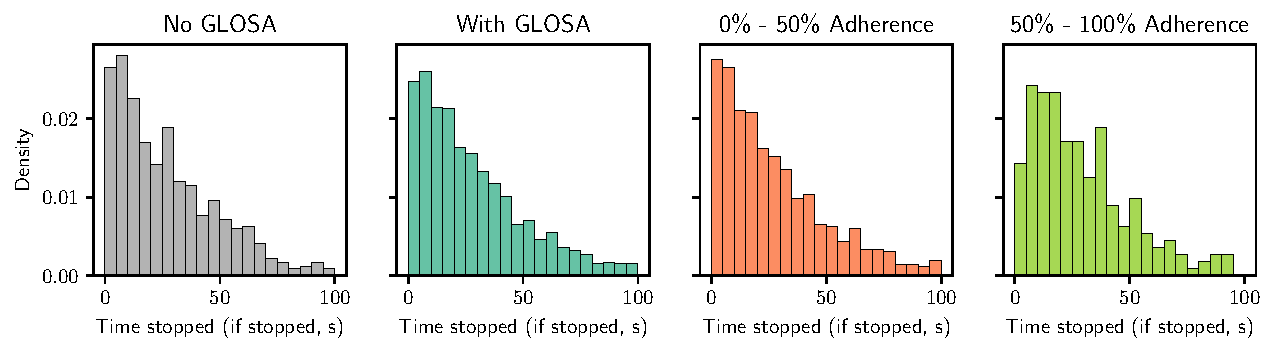
\includegraphics[width=\linewidth]{images/impacts-stop-time-adherence.pdf}
\end{figure}

\section{Conclusions}
